\chapter{First results and Future work}
\label{chap:results}

Although BERL is still in development and NeuroEvolution.jl is being tuned to reach decent performance, a few experiments have been conducted. 

\section{NEAT}

\begin{figure}[H]
\centering
\captionsetup{justification=centering,margin=2cm}
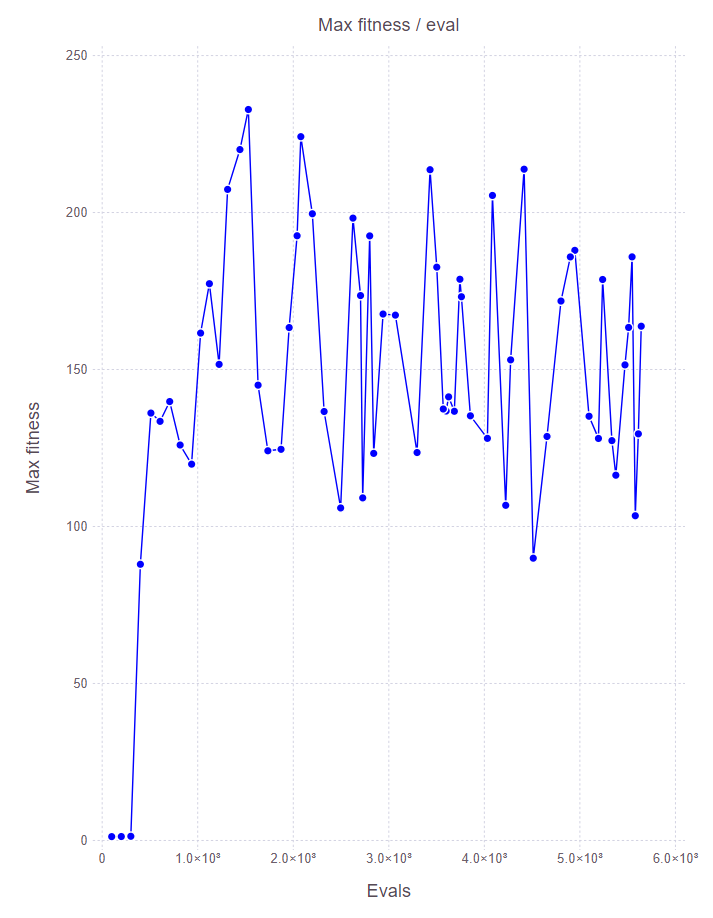
\includegraphics[height=8cm]{images/neat_antbullet.PNG}
\caption{NEAT run on an AntBullet environment: evolution of max fitness wrt the number of evaluations}
\end{figure}

A first experiment of NEAT on an AntBullet environment shows the algorithm learns and its maximum fitness improves, although it quickly stagnates as the best solutions seem to be forgotten between generations. This observation led to the implementation of elitism (cf section \ref{subsec:elitism}) to see if it improves performance in future experiments.

\section{Algorithm comparison}

We compared NEAT and CGP on the same CartPole benchmark. As the random seed of the environment is incremented at every generation, all individuals of a population are evaluated on the same environment but it changes between generations. This leads to a stochastic environment, hence even with elitism maximum fitness can decrease as the best individual in a generation may not perform as well on a slightly different environment. 

\begin{figure}[H]
\centering
\captionsetup{justification=centering,margin=2cm}
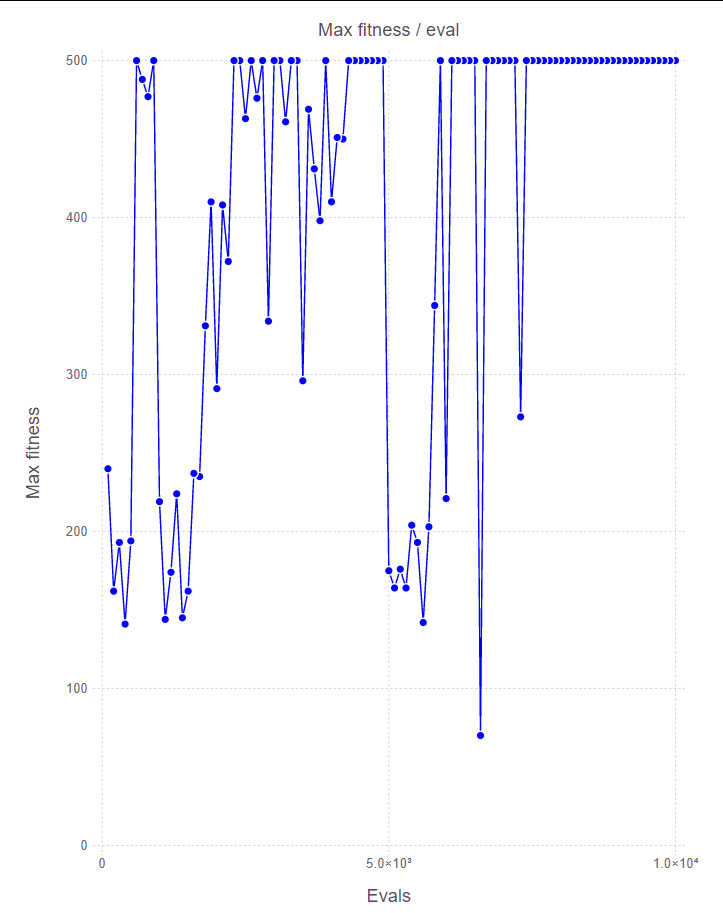
\includegraphics[height=10cm]{images/cgp_cartpole.PNG}
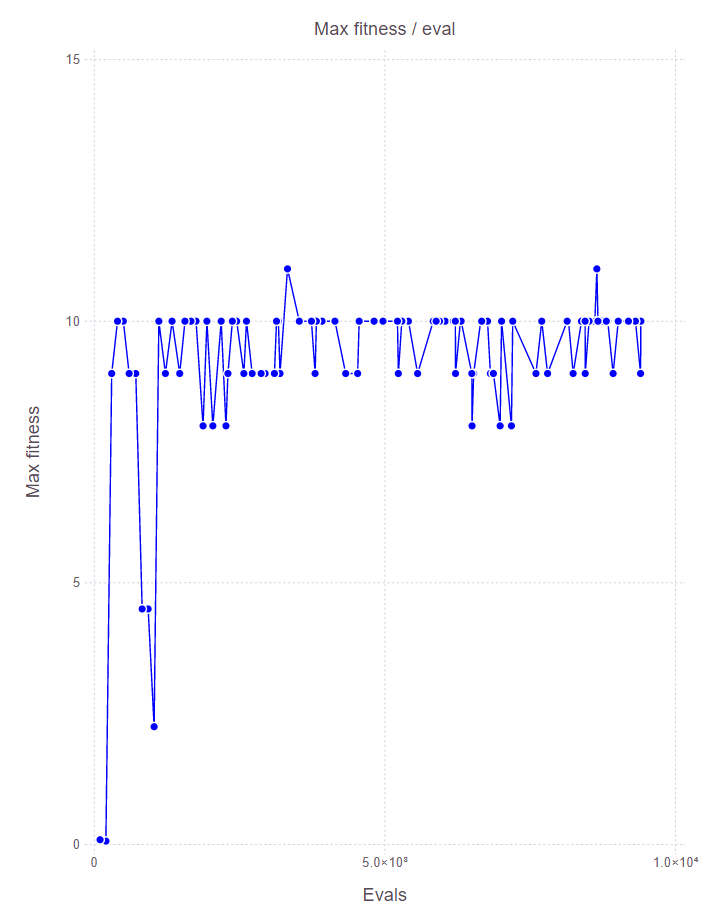
\includegraphics[height=10cm]{images/neat_cartpole.PNG}
\caption{CGP (left) and NEAT (right) runs on an Cartpole environment: evolution of max fitness wrt the number of evaluations}
\end{figure}

Although the environment is stochastic, hence harder to learn, CGP finally reaches a fitness of 100, solving the problem. However, NEAT (without elites) seems to struggle, showing further parameter tuning and features development are  still required. 


\section{Future work}

In the second part of this internship, I will keep developing NeuroEvolution.jl (\textit{NE.jl}) and BERL jointly in order both to provide more stable and efficient tools, and to use them as a platform to design, implement and benchmark new algorithms. 

In this regard, the following points are currently forecast to be essential components of my research work in the next months:
\begin{itemize}
    \item Adaptation of NE.jl and BERL.jl to Cambrian v0.2.0, which redefines the structure for a more robust and modular implementation
    \item Completion of the NEAT implementation with additional features as observed in the original code
    \item Development of a CMA-ES-optimized neural network in NE.jl for weight-only evolution
    \item Study of alternative indirect encoding algorithms, e.g. Artificial Gene Regulatory Networks \cite{GRN}
    \item Introduction of other evolutionary algorithmic mechanisms such as coevolution or Quality-Diversity in the NEAT structure
    \item Addition of gradient-based methods for weights optimization in a neuroevolution architecture
\end{itemize}

%%% Local Variables: 
%%% mode: latex
%%% TeX-master: "isae-report-template"
%%% End: 